\section{Multi-Foundation-Model Benchmarking}
\label{sec:benchmark}

\subsection{Purpose and comparison set}

This section compares pretrained tabular foundation models (TFMs) with conventional
prediction models using the same 17 clinical variables and the same held-out
real patients.  No synthetic records or precomputed embeddings are used.  The
diagnostic comparison includes logistic regression, XGBoost, TabPFN-3,
TabICLv2 and TabDPT.  The prognostic comparison includes elastic-net Cox
regression, a random survival forest, a TabPFN landmark adaptation and
SurvivalPFN.

The diagnostic question is whether the three classification foundation models
improve prediction of liver metastasis relative to logistic regression and
XGBoost.  The prognostic question is whether a classification foundation model
adapted to fixed survival horizons, or a model pretrained specifically for
right-censored survival data, improves prediction relative to Cox regression
and a random survival forest.  These are internal comparisons within the SEER
cohort; they do not replace the independent hospital validation of the
reference models presented earlier.

\noindent\textbf{Data used in this section.} All experiments use the 2 processed
real SEER datasets constructed in Section~\ref{sec:data}: the
2,672-patient diagnostic cohort and the 462-patient prognostic cohort. Models
receive the same 17 retained clinical predictors from these datasets. The
Erlangen cohort, the full-cohort synthetic datasets and the precomputed TabPFN
embeddings are not used in this benchmark. The test patients are real SEER
patients held out under the evaluation design described below.

All model specifications were fixed before evaluating the held-out patients.
The benchmark comprises 125 diagnostic fits: five models evaluated in five
repeats of five-fold cross-validation.  It also comprises 20 prognostic fits:
four models evaluated on five common 70/30 training--test partitions.  Every
fit completed and contributed to the reported results.

\subsection{Evaluation design}
\label{sec:benchmark:design}

For diagnosis, each cross-validation repeat gives every one of the 2,672
patients one prediction from a model that was not trained on that patient.
Performance was calculated separately in each repeat and then averaged across
the five repeats.  For prognosis, every partition contained 323 training and
139 test patients from the 462-patient cohort.  Performance was calculated in
each test set and averaged equally across the five partitions.

Preprocessing was fitted separately within each training partition.  This
included pooling categories represented by fewer than 15 training patients,
defining the category vocabulary, scaling continuous variables and removing
constant encoded columns.  The fitted transformation was then applied without
modification to the corresponding test patients.  Consequently, neither test
predictors nor test outcomes influenced model fitting or preprocessing.

Uncertainty was estimated from 2,000 patient-level bootstrap samples of the
held-out predictions.  The same resampled patients were used for all models,
which preserves the pairing needed for direct model comparisons.  Diagnostic
resampling retained the observed number of patients with and without liver
metastasis; prognostic resampling used the original patients and retained the
same patient weights wherever a patient appeared in a test partition.  The
reported 95\% percentile intervals therefore describe variation in the
evaluation patients while keeping the fitted models and data partitions
unchanged.  They do not include uncertainty from refitting, alternative model
seeds, pretraining or a different clinical population.  The intervals are
pointwise and were not adjusted for the number of comparisons.

\subsection{Models and implementation}

Table~\ref{tab:benchmark:identity} summarises the evaluated methods.  Logistic
and Cox regression used one-hot encoded categories, whereas the tree models and
foundation models used the training-derived ordinal representation.  All
models received the same underlying 17 clinical variables.

TabPFN-3, TabICLv2 and TabDPT are pretrained tabular classification models that
use the training table as context at prediction time rather than updating their
pretrained weights \citep{Hollmann2025,PriorLabsTabPFN3,Qu2026TabICLv2,Ma2025TabDPT}.
Their exact checkpoint versions were fixed and verified before evaluation.
The TabPFN landmark method fits separate TabPFN classifiers for death by 12,
24 and 36 months; it is therefore an adaptation of a classification model, not
a survival-pretrained model.  SurvivalPFN was pretrained for right-censored
time-to-event prediction and returns a survival distribution directly
\citep{Qi2026SurvivalPFN}.

\begin{table}[htbp]
\centering\scriptsize
\setlength{\tabcolsep}{3pt}
\caption{Models included in the matched benchmark.  One-hot and ordinal
encodings were learned separately within every training partition.  The
pretrained weights of the foundation models remained unchanged during
evaluation.}
\label{tab:benchmark:identity}
\begin{tabularx}{\linewidth}{@{}p{1.25cm}p{2.15cm}p{2.15cm}p{1.45cm}Y@{}}
\toprule
Task & Model & Model type & Clinical encoding & Main specification \\
\midrule
\csname @@input\endcsname{tables/multi_fm_benchmarking/model_identity_rows.tex}
\bottomrule
\end{tabularx}
\end{table}

All foundation models ran on the graphics processing unit (GPU).  Logistic
regression, XGBoost, Cox regression and the random survival forest ran on the
central processing unit (CPU).  Device choice was fixed for the experiment and
no automatic CPU fallback was allowed for a foundation model.

\FloatBarrier
\subsection{Diagnostic results}
\label{sec:benchmark:diagnostic}

Diagnostic performance was assessed with the area under the receiver operating
characteristic curve (ROC AUC), average precision and the Brier score.  ROC AUC
measures ranking across patients with and without liver metastasis.  Average
precision summarises the precision--recall relationship from the ranked
predictions \citep{SklearnAP}.  The Brier score is the mean squared error of the
predicted probabilities and is better when lower.

The three foundation models formed a narrow leading group
(Table~\ref{tab:benchmark:diagnostic}).  TabPFN-3 had the highest point ROC AUC
(0.903) and average precision (0.665).  TabICLv2 was nearly identical, with ROC
AUC 0.902, average precision 0.664 and the same rounded Brier score of 0.086.
TabDPT also reached ROC AUC 0.902.  Logistic regression remained competitive
at ROC AUC 0.895, whereas XGBoost reached 0.883.

\begin{table}[htbp]
\centering\scriptsize
\setlength{\tabcolsep}{3pt}
\caption{Diagnostic performance on held-out real patients.  ROC AUC, average
precision and Brier score are shown with pointwise 95\% patient-bootstrap
intervals.  Calibration slope and calibration-in-the-large intercept have
ideal values of 1 and 0, respectively.}
\label{tab:benchmark:diagnostic}
\begin{tabularx}{\linewidth}{@{}p{2.15cm}YYYrr@{}}
\toprule
Model & ROC AUC [95\% interval] & Average precision [95\% interval] & Brier score [95\% interval] & Slope & Intercept \\
\midrule
\csname @@input\endcsname{tables/multi_fm_benchmarking/diagnostic_performance_rows.tex}
\bottomrule
\end{tabularx}
\end{table}

The paired differences in Table~\ref{tab:benchmark:diagnostic-paired} show the
size and uncertainty of the changes relative to logistic regression.  The ROC
AUC improvements were 0.0088 for TabPFN-3, 0.0075 for TabICLv2 and 0.0074 for
TabDPT; all three intervals remained above zero.  Their Brier-score
improvements were also positive.  Average precision improved for TabPFN-3 and
TabICLv2, whereas the TabDPT interval included zero.  XGBoost was lower than
logistic regression in ROC AUC and Brier score, while its average-precision
interval included zero.

\begin{table}[htbp]
\centering\footnotesize
\caption{Paired diagnostic changes relative to logistic regression.  ROC AUC
and average precision are candidate minus logistic regression; Brier
improvement is logistic regression minus candidate.  Positive values favour
the listed model.  Intervals are pointwise and are not adjusted for multiple
comparisons.}
\label{tab:benchmark:diagnostic-paired}
\begin{tabularx}{\linewidth}{@{}p{2.5cm}YYY@{}}
\toprule
Model & $\Delta$ ROC AUC [95\% interval] & $\Delta$ average precision [95\% interval] & Brier improvement [95\% interval] \\
\midrule
\csname @@input\endcsname{tables/multi_fm_benchmarking/diagnostic_paired_rows.tex}
\bottomrule
\end{tabularx}
\end{table}

Calibration did not follow exactly the same ordering.  TabDPT had the slope
closest to one (1.001) and an intercept close to zero (0.008).  Logistic
regression also remained close to these targets (0.960 and 0.004).  TabPFN-3
and TabICLv2 had shallower slopes of 0.899 and 0.910 and positive intercepts of
0.091 and 0.084; XGBoost had the shallowest slope, 0.731.  The diagnostic result
is therefore a small foundation-model advantage in discrimination and overall
probability error, not a uniform improvement in calibration.

\begin{figure}[htbp]
\centering
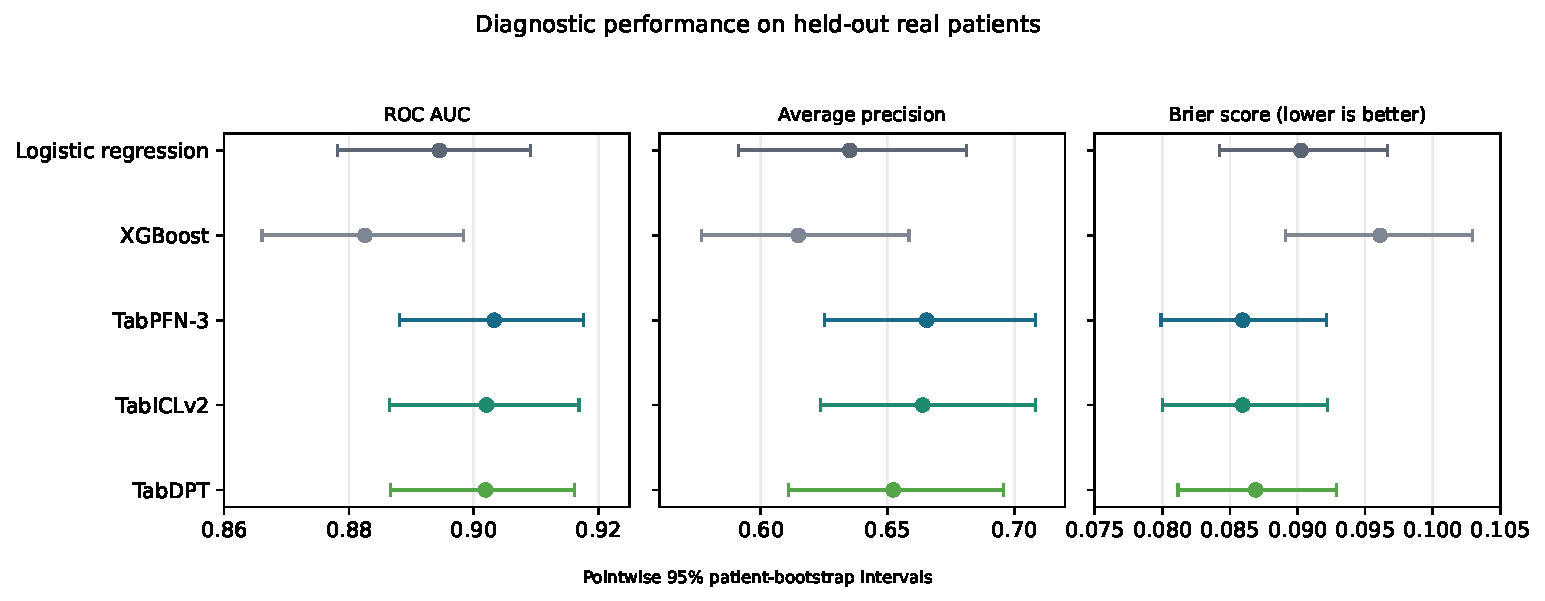
\includegraphics[width=\linewidth]{multi_fm_benchmarking/diagnostic_model_comparison.pdf}
\caption{Diagnostic performance on held-out real patients under the common
cross-validation design.  Points are the primary estimates and bars are
pointwise 95\% patient-bootstrap intervals.  Each panel has its own horizontal
scale; only the Brier score is better when lower.}
\label{fig:benchmark:diagnostic}
\end{figure}

\FloatBarrier
\subsection{Prognostic results}
\label{sec:benchmark:prognostic}

Prognostic discrimination was assessed with Uno's concordance index, which uses
inverse-probability-of-censoring weights to account for right censoring, and
with time-dependent ROC AUC at 12, 24 and 36 months
\citep{SksurvIPCW}.  The same censoring distribution, estimated from the real
training patients in each partition, was used for every model evaluated in that
partition.

The four models had similar discrimination (Table
\ref{tab:benchmark:prognostic-discrimination}).  Mean Uno concordance ranged
from 0.710 for SurvivalPFN to 0.717 for the TabPFN landmark method.  Every paired
concordance interval relative to Cox regression included zero.  Time-dependent
ROC AUC values ranged from 0.825 to 0.845 at 12 months and from 0.806 to 0.818 at
36 months.  These results do not show a clear discrimination advantage for any
foundation-model approach.

\begin{table}[htbp]
\centering\footnotesize
\caption{Prognostic discrimination on held-out real patients.  Uno concordance
is shown with its pointwise 95\% patient-bootstrap interval.  The horizon-specific
values are cumulative/dynamic ROC AUCs calculated from predicted death risk.}
\label{tab:benchmark:prognostic-discrimination}
\begin{tabularx}{\linewidth}{@{}p{3cm}Yrrr@{}}
\toprule
Model & Uno concordance [95\% interval] & ROC AUC 12 m & ROC AUC 24 m & ROC AUC 36 m \\
\midrule
\csname @@input\endcsname{tables/multi_fm_benchmarking/prognostic_discrimination_rows.tex}
\bottomrule
\end{tabularx}
\end{table}

The Brier score evaluates survival-probability error and is better when lower.
The integrated Brier score (IBS) summarises this error over the specified 12-,
24- and 36-month grid; it is not an integral over the complete follow-up period
\citep{SksurvIBS}.  The random survival forest had the lowest IBS (0.153),
followed by the TabPFN landmark method (0.155), Cox regression (0.160) and
SurvivalPFN (0.164).  Its paired IBS improvement over Cox regression was 0.0071
with a 95\% interval from 0.0012 to 0.0128 (Tables
\ref{tab:benchmark:prognostic-probability} and
\ref{tab:benchmark:prognostic-paired}).  The corresponding intervals for both
foundation-model approaches included zero.

For each model, the prognostic calibration summary divided test patients into
three equally sized groups according to predicted risk and compared mean
predicted survival with Kaplan--Meier (KM) survival at the three horizons.  All
15 partition--horizon summaries, each based on three risk groups, were
estimable for every model.  The random
survival forest had the smallest mean absolute gap (0.044), followed by
SurvivalPFN (0.052), the TabPFN landmark method (0.054) and Cox regression
(0.069).  These are descriptive summaries without comparative confidence
intervals, and each model defines its own risk groups.

\begin{table}[htbp]
\centering\footnotesize
\setlength{\tabcolsep}{3pt}
\caption{Prognostic probability error and grouped calibration.  Brier scores
and IBS are better when lower.  The Kaplan--Meier gap is the mean absolute
difference between predicted and observed survival across the 15 estimable
partition--horizon summaries, each based on three risk groups.}
\label{tab:benchmark:prognostic-probability}
\begin{tabularx}{\linewidth}{@{}p{2.8cm}rrrYr@{}}
\toprule
Model & Brier 12 m & Brier 24 m & Brier 36 m & IBS [95\% interval] & KM gap \\
\midrule
\csname @@input\endcsname{tables/multi_fm_benchmarking/prognostic_probability_rows.tex}
\bottomrule
\end{tabularx}
\end{table}

\begin{table}[htbp]
\centering\footnotesize
\caption{Paired prognostic changes relative to elastic-net Cox regression.
Uno concordance is candidate minus Cox; IBS improvement is Cox minus candidate.
Positive values favour the listed model.  The intervals are pointwise and are
not adjusted for multiple comparisons.}
\label{tab:benchmark:prognostic-paired}
\begin{tabularx}{\linewidth}{@{}p{4cm}YY@{}}
\toprule
Model & $\Delta$ Uno concordance [95\% interval] & IBS improvement [95\% interval] \\
\midrule
\csname @@input\endcsname{tables/multi_fm_benchmarking/prognostic_paired_rows.tex}
\bottomrule
\end{tabularx}
\end{table}

Although the random survival forest had a positive pointwise IBS interval
relative to Cox regression, the benchmark was not designed as a formal
multiple-comparison or superiority study.  The result supports a small
probability-error improvement within this evaluation, not universal superiority
of the random survival forest.  Likewise, intervals that include zero do not
establish that two methods are equivalent.

\begin{figure}[htbp]
\centering
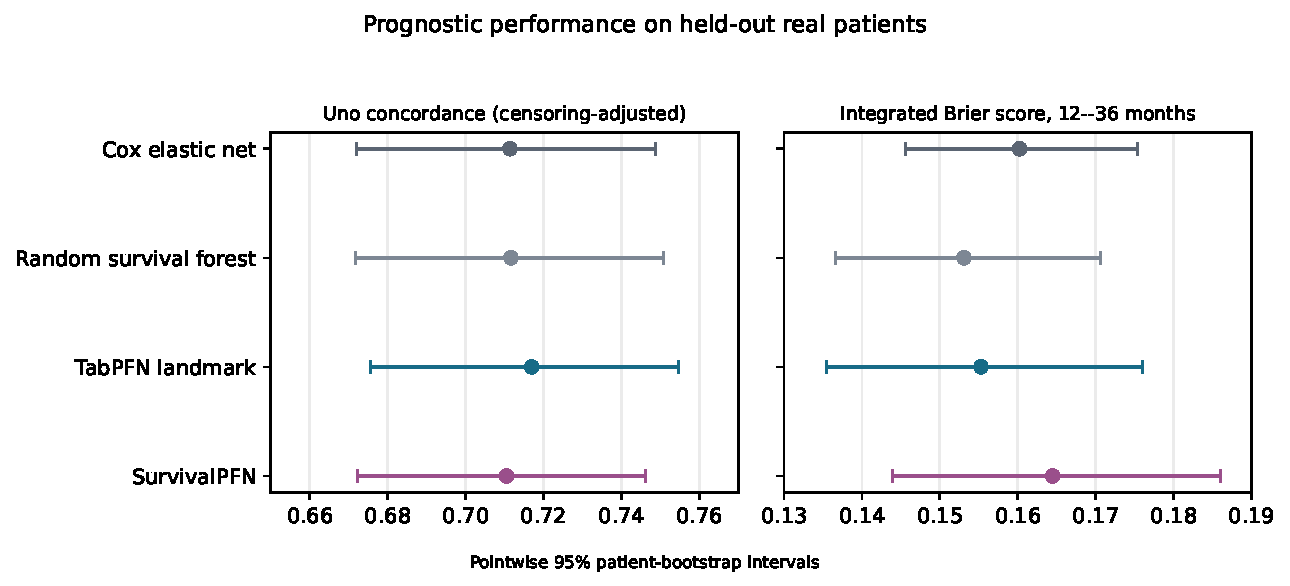
\includegraphics[width=0.86\linewidth]{multi_fm_benchmarking/prognostic_model_comparison.pdf}
\caption{Prognostic discrimination and probability error on held-out real
patients.  Points are primary estimates and bars are pointwise 95\%
patient-bootstrap intervals.  Higher Uno concordance and lower IBS are
favourable.}
\label{fig:benchmark:prognostic}
\end{figure}

\FloatBarrier
\subsection{Calibration and validity of survival predictions}
\label{sec:benchmark:calibration}

Figure~\ref{fig:benchmark:calibration} presents two different calibration
summaries.  The diagnostic panel shows the calibration slope calculated from
the out-of-fold probabilities, with an ideal value of one.  The prognostic
panel shows the mean absolute difference between predicted survival and
Kaplan--Meier survival in model-specific risk groups, with an ideal value of
zero.  Their numerical values should not be compared directly because they
measure different aspects of calibration.

\begin{figure}[htbp]
\centering
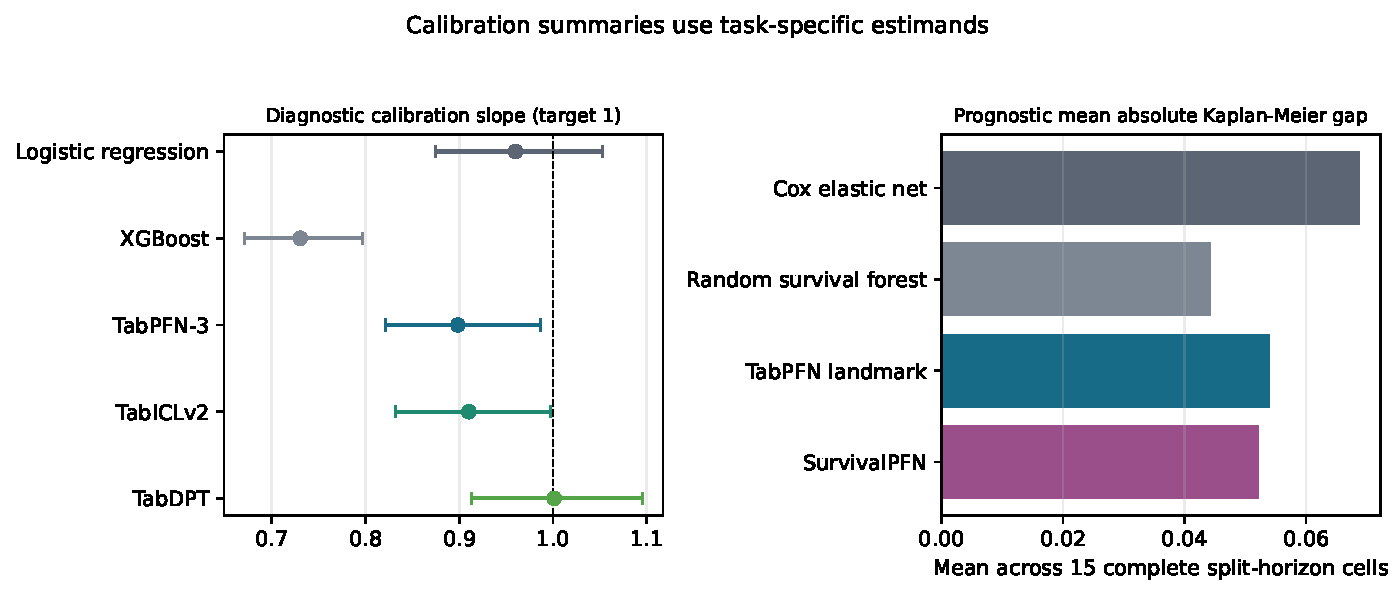
\includegraphics[width=0.88\linewidth]{multi_fm_benchmarking/calibration_summary.pdf}
\caption{Task-specific calibration summaries.  Diagnostic bars are pointwise
95\% patient-bootstrap intervals around the calibration slope, and the dashed
line marks the ideal value of one.  Prognostic bars are descriptive mean
absolute Kaplan--Meier gaps across 15 estimable partition--horizon comparisons
and have no confidence intervals.}
\label{fig:benchmark:calibration}
\end{figure}

The three TabPFN landmark classifiers predict survival independently at 12, 24
and 36 months.  They can therefore produce an invalid sequence in which
predicted survival increases at a later time.  This occurred in 41 of the 695
held-out prediction records and in every prognostic partition.  The unmodified
probabilities remain the primary results.  As a sensitivity analysis, each
patient's sequence was replaced by its cumulative minimum so that survival
could only remain constant or decrease.  This changed IBS only from 0.15529 to
0.15512.

SurvivalPFN returns a coherent survival distribution, but its predictions
changed slightly when the same test patients were arranged into different
query batches.  The largest observed change was 0.00035 in its risk score and
less than $10^{-6}$ in predicted survival.  To keep the calculation
reproducible, every test partition was scored once in a fixed patient order.

\FloatBarrier
\subsection{Computational profile}
\label{sec:benchmark:resources}

Table~\ref{tab:benchmark:resources} reports the median combined fitting and
prediction time for the real-data benchmark on the study computer.  Classical
models estimated new parameters in every training partition.  The foundation
models instead used each training table as context while keeping their
pretrained weights fixed.  The timings exclude environment setup, initial
checkpoint loading, bootstrap calculations and report preparation.  They
describe this hardware and implementation only; they are not general measures
of computational efficiency.

\begin{table}[htbp]
\centering\footnotesize
\setlength{\tabcolsep}{3pt}
\caption{Computational profile on the study computer.  Training/context rows
are the median number of real training patients supplied to each model.  Wall
time is the median combined fitting and prediction time per evaluation unit on
the RTX 3060 Laptop GPU and host CPU.}
\label{tab:benchmark:resources}
\begin{tabularx}{\linewidth}{@{}p{1.55cm}p{2.65cm}rrrrY@{}}
\toprule
Task & Model & Units & Device & Training/context rows & Median wall time (s) & Training behaviour \\
\midrule
\csname @@input\endcsname{tables/multi_fm_benchmarking/resource_rows.tex}
\bottomrule
\end{tabularx}
\end{table}

Median diagnostic times were 0.20 seconds for logistic regression, 0.28 for
XGBoost, 1.33 for TabDPT, 1.42 for TabICLv2 and 2.82 for TabPFN-3.  Median
prognostic times were 0.58 seconds for Cox regression, 0.73 for the random
survival forest, 5.81 for the three TabPFN landmark classifiers together and
6.80 for SurvivalPFN.  These results show that all methods were feasible on the
available 6-GB GPU system, but they do not measure energy use, checkpoint
loading latency or deployment throughput.

\FloatBarrier
\subsection{Interpretation and transition}
\label{sec:benchmark:limits}

The diagnostic results favour all three pretrained classification TFMs over
logistic regression in ROC AUC and Brier score, but the ROC AUC gains are small
(0.0074--0.0088).  TabPFN-3 and TabICLv2 also improve average precision, while
TabDPT has the calibration slope closest to one.  No model is best on every
criterion, and third-decimal differences should not be treated as a definitive
ranking.

No corresponding prognostic TFM advantage was demonstrated.  All four methods
have similar discrimination, and SurvivalPFN has neither the lowest IBS nor the
smallest grouped calibration gap.  This result applies to the evaluated cohort,
model specifications and five internal test partitions; it does not show that
survival pretraining is ineffective in other settings.

The main limitations are internal validation in one SEER extract, bootstrap
intervals that omit refitting and seed variability, and multiple pointwise
comparisons without adjustment or a predefined clinically important margin.
Checkpoint identities were verified, but the upstream development datasets
were not independently reconstructed.  The precomputed TabPFN embeddings were
excluded because they were created from the complete cohort before the
evaluation partitions and are reported separately as exploratory analyses.

Overall, the benchmark supports a modest diagnostic advantage for the three
classification TFMs, but no prognostic advantage over Cox regression or the
random survival forest.  Section~9 tests whether a trainable nonlinear
neural-network head changes either conclusion.
